% ថ្នាក់ទី ១១ (វិទ្យាសាស្ត្រ) · ជំពូកទី ៨ · មេរៀនទី ១ · សៀវភៅភាគ ២ ទំព័រ ១៥៩–១៦៩
\chapter{រូបធរណីមាត្រក្នុងលំហ}

\begin{note}[ជំពូកទី ៨ ៖ ធរណីមាត្រក្នុងលំហ]
ជំពូកនេះមានមេរៀន ៖ \textbf{១. រូបធរណីមាត្រក្នុងលំហ} \quad \textbf{២. បន្ទាត់និងប្លង់ស្របក្នុងលំហ} \quad \textbf{៣. ភាពអរត្តូកូណាល់ក្នុងលំហ} ។

អេស៊ីប (Egypt) ជាប្រទេសមួយសំបូរទៅដោយសំណង់ពីរ៉ាមីតជាច្រើន ប៉ុន្តែក្នុងបណ្ដាពីរ៉ាមីតទាំងនេះមានតែពីរ៉ាមីតឈ្មោះ Giza ប៉ុណ្ណោះដែលមានវ័យចំណាស់ ហើយធំជាងគេនៅលើពិភពលោក ។ ពីរ៉ាមីតនេះកាលពីមុនវាមានកម្ពស់ $146.6$ m ឥឡូវនៅសល់តែ $138.8$ m ហើយបានសាងសង់នៅឆ្នាំ $2570$ មុនគ្រិស្តសករាជ បេតិកភណ្ឌពីរ៉ាមីតនេះ បានផ្ដល់នូវគំនិតជាច្រើនសម្រាប់ការសិក្សាធរណីមាត្រក្នុងលំហ ។
\end{note}

\begin{objBox}[វត្ថុបំណង]
\begin{enumerate}[1]
  \item គូសរូបក្នុងលំហនៅលើប្លង់
  \item ប្រាប់បានពីស្វ័យសត្យបន្ទាត់ ស្វ័យសត្យប្លង់
  \item កំណត់ប្លង់បាន
  \item បង្ហាញថាបន្ទាត់មួយនៅក្នុងប្លង់ឬមិននៅក្នុងប្លង់
  \item កំណត់ប្លង់ពីរប្រសព្វគ្នា
  \item កំណត់ទីតាំងបន្ទាត់និងបន្ទាត់ បន្ទាត់និងប្លង់ ប្លង់និងប្លង់ក្នុងលំហ ។
\end{enumerate}
\end{objBox}

\section{ការគូសរូបក្នុងលំហនៅលើប្លង់}
នៅក្នុងជីវភាពរស់នៅ មានវត្ថុជាច្រើនជារូបធរណីមាត្រក្នុងលំហ ។ គេចង់គូសរូបទាំងនេះនៅលើផ្ទៃរាប ដែលជាប្លង់មួយ ។

\begin{example}[ឧទាហរណ៍]
គេចង់គូសរូបគូបមួយក្នុងផ្ទៃរាបដែលជាប្លង់មួយហើយ ដើម្បីឱ្យរូបនេះបង្ហាញឱ្យឃើញវិមាត្រនៃបាតនិងកម្ពស់នៃគូប ដូច្នេះគេប្រើវិធីដូចខាងក្រោម ៖
\end{example}
\begin{center}
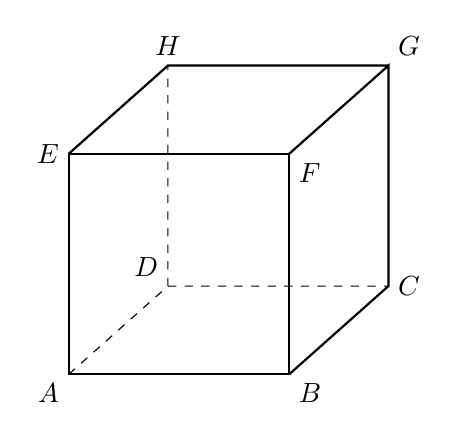
\begin{tikzpicture}[scale=1.4]
\coordinate (A) at (0,0); \coordinate (B) at (2,0); \coordinate (C) at (2.9,0.8); \coordinate (D) at (0.9,0.8);
\coordinate (E) at (0,2); \coordinate (F) at (2,2); \coordinate (G) at (2.9,2.8); \coordinate (H) at (0.9,2.8);
\draw[thick] (A) -- (B) -- (F) -- (E) -- cycle;
\draw[thick] (B) -- (C) -- (G) -- (F) (E) -- (H) -- (G);
\draw[dashed] (A) -- (D) -- (C) (D) -- (H);
\foreach \p/\a in {A/below left,B/below right,C/right,D/above left,E/left,F/below right,G/above right,H/above} \node[\a] at (\p) {$\p$};
\end{tikzpicture}
\end{center}
\begin{itemize}
  \item គ្រប់ទ្រនុងស្របគ្នាទាំងអស់នៃគូប គឺគូសដោយបន្ទាត់ស្របគ្នា ។ ចំពោះទ្រនុងដែលគេមើលឃើញ ត្រូវគូសដោយគំនូសជាប់ ។ ចំពោះទ្រនុងដែលបាំងត្រូវគូសដោយគំនូសដាច់ ។
  \item មុខ $ABFE$ ដែលគេមើលឃើញចំពីមុខវានៅរក្សារាងដើមជាការេដដែល ។
  \item មុខ $BCGF$ និង $ADHE$ ជាមុខដែលគេមើលពីចំហៀង ។
\end{itemize}
ដូច្នេះ មុំត្រូវខុសពីទម្រង់ដើមហើយទ្រនុងខ្លះអាចខុសពីប្រវែងពិតរបស់វា ។ ក្នុងករណីនេះមុខទាំងនោះតាងដោយប្រលេឡូក្រាម ។

\begin{theorem}[សន្និដ្ឋាន]
\begin{enumerate}[1]
  \item ដើម្បីគូសរូបក្នុងលំហ គេត្រូវស្គាល់ច្បាស់អំពីទ្រង់ទ្រាយដើម
  \item បន្ទាត់ស្របគ្នាក្នុងលំហ តាងដោយបន្ទាត់ស្របគ្នាក្នុងប្លង់
  \item អង្កត់ពីរដែលមានប្រវែងស្មើគ្នានៅក្នុងលំហអាចមិនចាំបាច់ តាងដោយអង្កត់ពីរដែលមានប្រវែងស្មើគ្នានៅក្នុងប្លង់ទេ ។
\end{enumerate}
\end{theorem}

\begin{pro}
គូសរូបឡើងវិញដោយអង្កត់ដាច់ៗឱ្យបានត្រឹមត្រូវ ៖ ក. ប្រលេពីប៉ែតកែង \quad ខ. ពីរ៉ាមីតបាតការេ \quad គ. រូបផ្គុំដោយគូបបី ។
\ans
គូសទ្រនុងដែលមើលឃើញដោយគំនូសជាប់ និងទ្រនុងដែលបាំងដោយគំនូសដាច់ ។ ឧទាហរណ៍សម្រាប់ ក និង ខ ៖
\begin{center}
\begin{tikzpicture}[scale=0.9]
\draw[thick] (0,0) -- (1.6,0) -- (1.6,2.6) -- (0,2.6) -- cycle;
\draw[thick] (1.6,0) -- (2.4,0.7) -- (2.4,3.3) -- (0.8,3.3) -- (0,2.6) (1.6,2.6) -- (2.4,3.3);
\draw[dashed] (0,0) -- (0.8,0.7) -- (2.4,0.7) (0.8,0.7) -- (0.8,3.3);
\node at (1.2,-0.5) {ក.};
\begin{scope}[xshift=4cm]
\coordinate (a) at (0,0); \coordinate (b) at (2,0); \coordinate (c) at (2.8,0.8); \coordinate (d) at (0.8,0.8); \coordinate (s) at (1.4,3);
\draw[thick] (a) -- (b) -- (c) -- (s) -- cycle (b) -- (s);
\draw[dashed] (a) -- (d) -- (c) (d) -- (s) (s) -- (1.4,0.4);
\draw (1.4,0.4) -- ++(0.2,0) -- ++(0,0.2);
\node at (1.4,-0.5) {ខ.};
\end{scope}
\end{tikzpicture}
\end{center}
\end{pro}

\begin{pro}
សង់រូបដែលកើតបានពីការបង្វិលរូបនីមួយៗខាងក្រោមជុំវិញអ័ក្ស $XY$ ត្រូវនឹងមុំ $360^\circ$ ៖ ក. ត្រីកោណកែង $OHA$ (កែងត្រង់ $H$) ដែល $OH$ នៅលើ $XY$ \quad ខ. ចតុកោណកែង $OABO'$ ដែល $OO'$ នៅលើ $XY$ ។
\ans
ក. កោណបរិវត្តន៍ដែលមានកំពូល $O$ កម្ពស់ $OH$ និងកាំបាត $HA$ ។ \quad ខ. ស៊ីឡាំងបរិវត្តន៍ដែលមានកម្ពស់ $OO'$ និងកាំបាត $OA = O'B$ ។
\begin{center}
\begin{tikzpicture}[scale=0.8]
\draw[thick] (-1.5,0) -- (0,3) -- (1.5,0);
\draw[thick] (-1.5,0) arc (180:360:1.5 and 0.35);
\draw[dashed] (1.5,0) arc (0:180:1.5 and 0.35);
\draw[dashed] (0,0) -- (0,3) (0,0) -- (1.5,0);
\node[above] at (0,3) {$O$}; \node[below] at (0,-0.35) {ក.};
\begin{scope}[xshift=4.5cm]
\draw[thick] (-1.3,0) -- (-1.3,3) (1.3,0) -- (1.3,3);
\draw[thick] (0,3) ellipse (1.3 and 0.3);
\draw[thick] (-1.3,0) arc (180:360:1.3 and 0.3);
\draw[dashed] (1.3,0) arc (0:180:1.3 and 0.3);
\draw[dashed] (0,0) -- (0,3);
\node[above] at (0,3.3) {$O$}; \node[below] at (0,-0.35) {ខ.};
\end{scope}
\end{tikzpicture}
\end{center}
\end{pro}

\section{លក្ខណៈគ្រឹះ}
\subsection{ស្វ័យសត្យបន្ទាត់}
គេយកអំបោះពីរសរសៃទៅពាក់សន្ទឹងពីលើម្ជុលបារាំងពីរ $A$ និង $B$ ដែលគេដោតជាប់នឹងបន្ទះក្ដារមួយ ។ គេឃើញថាអំបោះទាំងពីរសរសៃនេះត្រួតស៊ីគ្នា ។
\begin{theorem}[ស្វ័យសត្យ]
តាមពីរចំណុចផ្សេងគ្នា គេអាចគូសបន្ទាត់បានតែមួយគត់ ។
\end{theorem}

\subsection{ស្វ័យសត្យប្លង់}
ជាងឈើម្នាក់ធ្វើតុមួយមានជើងបី ហើយគាត់យកតុនេះទៅដាក់លើផ្ទៃរាបមួយ គេសង្កេតឃើញថាតុមានលំនឹងល្អ ។
\begin{theorem}[ស្វ័យសត្យ]
តាមបីចំណុចមិនស្ថិតលើបន្ទាត់តែមួយ គេអាចកំណត់បានប្លង់តែមួយគត់ ។
\end{theorem}

\subsection{ការកំណត់ប្លង់}
តាមស្វ័យសត្យប្លង់ គេអាចកំណត់ប្លង់បានដូចខាងក្រោម ៖
\begin{center}
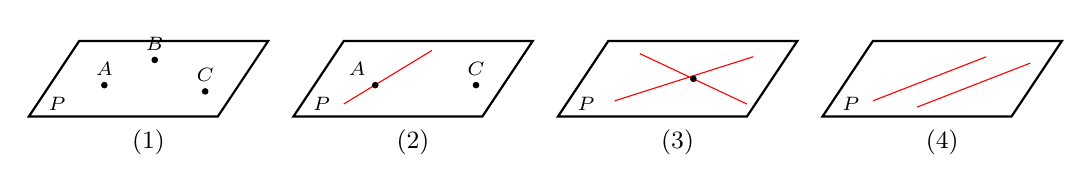
\begin{tikzpicture}[scale=0.8]
\foreach \x/\t in {0/1,4.2/2,8.4/3,12.6/4} {
  \begin{scope}[xshift=\x cm]
  \draw[thick] (0,0) -- (3,0) -- (3.8,1.2) -- (0.8,1.2) -- cycle;
  \node at (0.45,0.2) {\scriptsize $P$};
  \node at (1.9,-0.4) {\small (\t)};
  \end{scope}}
\fill (1.2,0.5) circle (1.5pt) node[above] {\scriptsize $A$}; \fill (2,0.9) circle (1.5pt) node[above] {\scriptsize $B$}; \fill (2.8,0.4) circle (1.5pt) node[above] {\scriptsize $C$};
\draw[red] (4.2+0.8,0.2) -- (4.2+2.2,1.05); \fill (4.2+1.3,0.5) circle (1.5pt) node[above left] {\scriptsize $A$}; \fill (4.2+2.9,0.5) circle (1.5pt) node[above] {\scriptsize $C$};
\draw[red] (8.4+0.9,0.25) -- (8.4+3.1,0.95) (8.4+1.3,1.0) -- (8.4+3.0,0.2); \fill (8.4+2.15,0.6) circle (1.5pt);
\draw[red] (12.6+0.8,0.25) -- (12.6+2.6,0.95) (12.6+1.5,0.15) -- (12.6+3.3,0.85);
\end{tikzpicture}
\end{center}
\begin{formulaBox}[ការកំណត់ប្លង់]
\begin{enumerate}[1]
  \item បីចំណុចដែលមិនស្ថិតនៅលើបន្ទាត់តែមួយកំណត់បានប្លង់តែមួយគត់ ។
  \item បន្ទាត់មួយ និងចំណុចមួយដែលមិនស្ថិតលើបន្ទាត់នោះ កំណត់បានប្លង់មួយគត់ ។
  \item បន្ទាត់ពីរប្រសព្វគ្នា កំណត់បានប្លង់មួយ ។
  \item បន្ទាត់ពីរស្របគ្នា កំណត់បានប្លង់មួយ ។
\end{enumerate}
\end{formulaBox}

\begin{example}[លំហាត់គំរូ ១]
គេមានបួនចំណុច $A, B, C$ និង $D$ មិនស្ថិតក្នុងប្លង់តែមួយ ។ កំណត់ប្លង់ទាំងអស់ដែលកំណត់ដោយចំណុចបីៗ ។
\ans
តាមស្វ័យសត្យប្លង់គេបានប្លង់ $ABC$, $ABD$, $DBC$ និង $ACD$ ។
\end{example}
\begin{note}[សម្គាល់]
រូបធរណីមាត្រ $ABCD$ ហៅថា \textbf{ចតុមុខ} ឬ\textbf{តេត្រាអែត} ។
\end{note}
\begin{center}
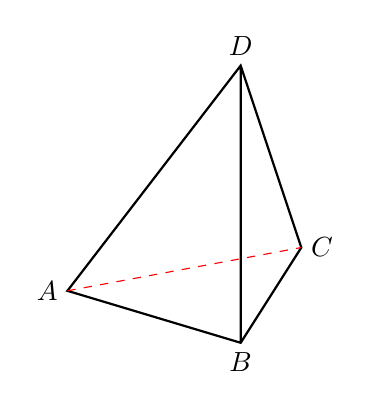
\begin{tikzpicture}[scale=1.1]
\coordinate (A) at (0,0); \coordinate (B) at (2,-0.6); \coordinate (C) at (2.7,0.5); \coordinate (D) at (2,2.6);
\draw[thick] (A) -- (B) -- (C) -- (D) -- cycle (B) -- (D);
\draw[dashed,red] (A) -- (C);
\node[left] at (A) {$A$}; \node[below] at (B) {$B$}; \node[right] at (C) {$C$}; \node[above] at (D) {$D$};
\end{tikzpicture}
\end{center}

\begin{pro}
គេឱ្យការេ $ABCD$ និង ចំណុច $O$ មួយស្ថិតនៅខាងក្រៅប្លង់នៃការេនេះ ។ តើតាមចំណុច $O$ គេអាចគូសបានប្លង់ប៉ុន្មាន ជាមួយនឹងជ្រុងនៃការេនោះ?
\ans
$4$ ប្លង់ ($OAB$, $OBC$, $OCD$, $ODA$) ។
\end{pro}

\textbf{អនុវត្តន៍ ៖} គេធ្វើទម្រនៃម៉ាស៊ីនថតរូបមានជើងបី ទើបមានលំនឹងល្អ ពីព្រោះចុងនៃជើងម៉ាស៊ីនថតរូបស្ថិតក្នុងប្លង់តែមួយ (តាមចំណុចបីរត់មិនត្រង់គ្នាគេគូសបានប្លង់តែមួយគត់) ។ ផ្ទុយទៅវិញ បើទម្រវាមានជើងបួន ចុងនៃជើងម៉ាស៊ីនថតរូបអាចស្ថិតនៅលើប្លង់ច្រើន ក្នុងករណីនេះជើងម៉ាស៊ីនថតរូបមិនអាចមានលំនឹងល្អបានទេ ។

\begin{example}[លំហាត់គំរូ ២]
គេឱ្យ $A, B, C, D$ ជាចំណុចនៅលើបន្ទាត់ $a$ មួយ ដែលមិនស្រប និងមិនកាត់ទៅនឹងបន្ទាត់ $\Delta$ ។ តើគេអាចកំណត់បានប្លង់ប៉ុន្មាន ដែលកាត់តាមបន្ទាត់ $\Delta$ និងចំណុចនីមួយៗ?
\ans
តាមការកំណត់នៃប្លង់ បន្ទាត់មួយ និងចំណុចមួយមិនស្ថិតលើបន្ទាត់តែមួយ កំណត់បានប្លង់មួយគត់ ។ ដូច្នេះ គេអាចកំណត់បានប្លង់បួនគឺ ៖ ប្លង់ដែលមាន $A$ ជាមួយនឹង $\Delta$, ប្លង់ដែលមាន $B$ ជាមួយនឹង $\Delta$, ប្លង់ដែលមាន $C$ ជាមួយនឹង $\Delta$ និងប្លង់ដែលមាន $D$ ជាមួយនឹង $\Delta$ ។
\end{example}

\begin{pro}
គេមានបីបន្ទាត់ $d_1$, $d_2$ និង $d_3$ ដែល $d_1 \parallel d_2 \parallel d_3$ នៅក្នុងប្លង់ $P$ មួយ និងបន្ទាត់ $d$ មិនស្ថិតក្នុងប្លង់ $P$ តែស្របទៅនឹងបន្ទាត់ទាំងបីខាងលើ ។ តើតាមបន្ទាត់ $d_1$, $d_2$ និង $d_3$ គេអាចកំណត់បានប្លង់ប៉ុន្មានជាមួយនឹងបន្ទាត់ $d$?
\ans
$3$ ប្លង់ ។
\end{pro}

\subsection{បន្ទាត់នៅក្នុងប្លង់}
គេដៅចំណុចពីរ $A$ និង $B$ នៅលើប្លង់ក្ដារខៀនឬក្រដាសមួយរួចយកបន្ទាត់មួយដាក់ឱ្យកាត់តាមពីរចំណុចនេះ យើងបានបន្ទាត់នេះស្ថិតជាប់នឹងផ្ទៃក្ដារខៀនឬក្រដាស ។ គេថាបន្ទាត់នេះស្ថិតក្នុងប្លង់ក្ដារខៀនឬក្រដាស ។
\begin{theorem}[លក្ខណៈ]
បើបន្ទាត់មួយ និងប្លង់មួយមានចំណុចរួមពីរផ្សេងគ្នា នោះបន្ទាត់ស្ថិតក្នុងប្លង់នោះ ៖
\[
\left.\begin{aligned} A, B &\in P\\ A, B &\in L \end{aligned}\right\} \Rightarrow L \subset P
\]
\end{theorem}

\begin{example}[លំហាត់គំរូ]
គេមានបួនចំណុច $A, B, C, D$ ក្នុងប្លង់ $P$ ដែលបីចំណុចមិនស្ថិតនៅលើបន្ទាត់តែមួយ ។ តើតាមបួនចំណុចនេះ គេអាចគូសបានបន្ទាត់ដែលស្ថិតនៅក្នុងប្លង់ $P$ បានប៉ុន្មាន?
\ans
គេដឹងថាតាមពីរចំណុចផ្សេងគ្នា គេអាចគូសបន្ទាត់បានតែមួយគត់ ។ ដូច្នេះ តាមបួនចំណុច $A, B, C, D$ មិនស្ថិតលើបន្ទាត់តែមួយ គេអាចគូសបានបន្ទាត់ចំនួន $6$ គឺបន្ទាត់ $AB$, $AC$, $AD$, $BC$, $BD$, $CD$ ។
\end{example}

\begin{pro}
គេមានប្រាំចំណុច $A, B, C, D, E$ ក្នុងប្លង់ $P$ ដែលចំណុចបីៗមិនស្ថិតនៅលើបន្ទាត់តែមួយ ។ តើតាមប្រាំចំណុចនេះអាចគូសបានបន្ទាត់ដែលស្ថិតនៅក្នុងប្លង់ $P$ បានប៉ុន្មាន?
\ans
${}_5C_2 = 10$ បន្ទាត់ ។
\end{pro}

\subsection{ប្រសព្វរវាងប្លង់និងប្លង់}
ការបើកសៀវភៅអាន ឬការធ្វើជញ្ជាំងផ្ទះអាចផ្ដល់ជារូបភាពប្លង់ពីរប្រសព្វគ្នាតាមបន្ទាត់មួយ ។ គេមានចំណុច $A$ នៅក្នុងប្លង់ $P$ មួយ និងបន្ទាត់ $BC$ នៅក្រៅប្លង់ $P$ ។ បន្លាយ $BA$ ហើយជ្រើសរើសចំណុច $F$ នៅលើ $BA$ ឱ្យបាន $AF$ ។ រួចភ្ជាប់ពីចំណុច $C$ មក $F$ កាត់ប្លង់ $P$ ត្រង់ $G$ ។ គេបានចំណុច $A, G$ ទាំងពីរស្ថិតក្នុងប្លង់ $ABC$ និងប្លង់ $P$ ។ ដូច្នេះ គេបានបន្ទាត់ $AG$ ជាបន្ទាត់រួមនៃប្លង់ $ABC$ និងប្លង់ $P$ ។
\begin{theorem}[សន្និដ្ឋាន]
បើប្លង់ពីរមានចំណុចរួមមួយ វាប្រសព្វគ្នាតាមបន្ទាត់មួយដែលកាត់តាមចំណុចរួមនោះ ។
\end{theorem}

\begin{example}[លំហាត់គំរូ]
ក្នុងរូបធរណីមាត្រ (ចតុមុខ $ABCD$) $B' \in BD$ និង $C' \in DC$ ដែល $B'C'$ មិនស្របនឹង $BC$ កំណត់ប្រសព្វរវាងប្លង់ $ABC$ និង $AB'C'$ ។
\ans
គេឃើញថាប្លង់ $ABC$ និង $AB'C'$ មាន $A$ ជាចំណុចរួម ។ ហេតុនេះត្រូវរកចំណុចរួមមួយទៀត ។ គូសបន្ទាត់ $BC$ និង $B'C'$ ដែលកាត់គ្នាត្រង់ $E$ ។
\[
\left.\begin{aligned} E &\in B'C'\\ B'C' &\subset AB'C' \end{aligned}\right\} \Rightarrow E \in AB'C'
\qquad
\left.\begin{aligned} E &\in BC\\ BC &\subset ABC \end{aligned}\right\} \Rightarrow E \in ABC
\]
ដូច្នេះ $AE$ ជាប្រសព្វរវាងប្លង់ $ABC$ និង $AB'C'$ ។
\begin{center}
\begin{tikzpicture}[scale=1.2]
\coordinate (B) at (0,0); \coordinate (C) at (2,-0.4); \coordinate (A) at (2.8,0.5); \coordinate (D) at (2.1,2.6);
\coordinate (Bp) at ($(B)!0.55!(D)$); \coordinate (Cp) at ($(C)!0.35!(D)$);
\coordinate (E) at (-2.4,0.48);
\draw[thick] (B) -- (C) -- (A) -- (D) -- cycle (C) -- (D);
\draw[dashed] (B) -- (A);
\draw[red] (E) -- (B) (E) -- (Bp) -- (Cp);
\draw[red,dashed] (E) -- (A) (Bp) -- (A) (Cp) -- (A);
\foreach \p/\l/\a in {A/A/right,B/B/below,C/C/below,D/D/above,Bp/B'/above left,Cp/C'/right,E/E/left} \node[\a] at (\p) {$\l$};
\end{tikzpicture}
\end{center}
\end{example}

\begin{pro}
នៅក្នុងប្លង់ $P$ មានការេ $ABCD$ មួយ ។ ចំណុច $O$ មួយនៅក្រៅប្លង់ $P$ ។
\begin{enumerate}[a]
  \item កំណត់ប្រសព្វរវាងប្លង់ $OAC$ និង $OBD$ ។
  \item $A'$ កណ្ដាលនៃ $OA$ ចូរកំណត់ប្រសព្វរវាងប្លង់ $A'BC$ និង $OAD$, $A'BC$ និង $ODC$ ។
\end{enumerate}
\ans
ក. តាង $I = AC \cap BD$ (ផ្ចិតការេ) ។ ប្លង់ទាំងពីរមាន $O$ និង $I$ ជាចំណុចរួម ដូច្នេះប្រសព្វគឺបន្ទាត់ $OI$ ។ \quad ខ. ដោយ $BC \parallel AD$ ប្រសព្វនៃប្លង់ $A'BC$ និង $OAD$ គឺបន្ទាត់កាត់តាម $A'$ ហើយស្របនឹង $AD$ ដែលកាត់ $OD$ ត្រង់ $D'$ កណ្ដាលនៃ $OD$ គឺ $A'D'$ ។ ដូច្នេះប្លង់ $A'BC$ គឺប្លង់ $A'BCD'$ ហើយប្រសព្វនៃ $A'BC$ និង $ODC$ គឺបន្ទាត់ $CD'$ ។
\end{pro}

\section{ទីតាំងរវាងបន្ទាត់និងប្លង់}
\subsection{ទីតាំងរវាងបន្ទាត់ពីរក្នុងលំហ}
\textbf{បន្ទាត់ពីរប្រសព្វគ្នានៅក្នុងប្លង់តែមួយ ៖} បន្ទាត់ពីរប្រសព្វគ្នាត្រង់មួយចំណុច នៅក្នុងប្លង់តែមួយ ។ បន្ទាត់ $d_1$ និង $d_2$ ប្រសព្វគ្នាត្រង់ចំណុច $I$ មួយ ។ គេកំណត់សរសេរ $d_1 \cap d_2 = \{I\}$ ។

\textbf{បន្ទាត់ពីរស្របគ្នានៅក្នុងប្លង់តែមួយ ៖} បន្ទាត់ $d_1$ និង $d_2$ គ្មានចំណុចរួម គេថាបន្ទាត់ $d_1$ ស្រប $d_2$ ។ គេកំណត់សរសេរ $d_1 \parallel d_2$ ។

\textbf{បន្ទាត់ពីរមិនប្រសព្វនិងមិនស្របគ្នា ៖} បន្ទាត់ពីរមិនប្រសព្វ និងមិនស្របគ្នា គឺមិនអាចនៅក្នុងប្លង់តែមួយទេ ។ គេកំណត់សរសេរ $\begin{cases} d_1 \cap d_2 = \varnothing\\ d_1 \nparallel d_2 \end{cases}$ ។
\begin{center}
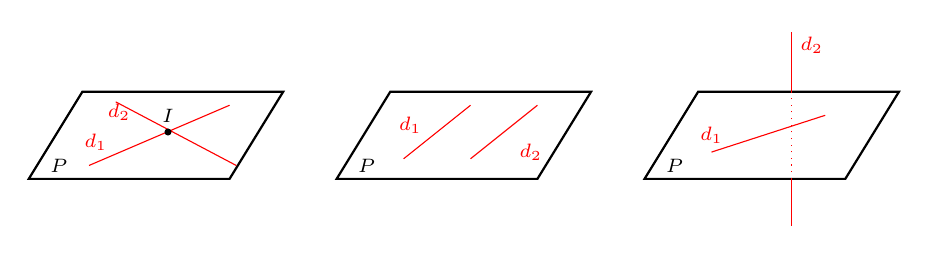
\begin{tikzpicture}[scale=0.85]
\foreach \x in {0,4.6,9.2} {\draw[thick] (\x,0) -- (\x+3,0) -- (\x+3.8,1.3) -- (\x+0.8,1.3) -- cycle; \node at (\x+0.45,0.2) {\scriptsize $P$};}
\draw[red] (0.9,0.2) -- (3.0,1.1) (1.3,1.15) -- (3.1,0.2); \fill (2.08,0.7) circle (1.5pt) node[above] {\scriptsize $I$};
\node[red] at (1,0.55) {\scriptsize $d_1$}; \node[red] at (1.35,1.0) {\scriptsize $d_2$};
\draw[red] (4.6+1.0,0.3) -- (4.6+2.0,1.1) (4.6+2.0,0.3) -- (4.6+3.0,1.1); \node[red] at (4.6+1.1,0.8) {\scriptsize $d_1$}; \node[red] at (4.6+2.9,0.4) {\scriptsize $d_2$};
\draw[red] (9.2+1.0,0.4) -- (9.2+2.7,0.95); \node[red] at (9.2+1.0,0.65) {\scriptsize $d_1$};
\draw[red] (9.2+2.2,1.3) -- (9.2+2.2,2.2) (9.2+2.2,0) -- (9.2+2.2,-0.7); \draw[red,dotted] (9.2+2.2,0) -- (9.2+2.2,1.3); \node[red] at (9.2+2.5,2.0) {\scriptsize $d_2$};
\end{tikzpicture}
\end{center}

\textbf{មុំបង្កើតដោយបន្ទាត់ពីរក្នុងលំហ ៖} ក្នុងករណីបន្ទាត់ពីរ $d'$ និង $d$ មិនប្រសព្វ និងមិនស្របគ្នាគេអាចកំណត់មុំដែលផ្គុំដោយបន្ទាត់ទាំងពីរនេះបាន ។ ដំបូងគេគូសបន្ទាត់ $d'_1$ មួយផ្សេងទៀតឱ្យស្របទៅនឹង $d'$ ហើយកាត់បន្ទាត់ $d$ ត្រង់ចំណុចណាមួយដែលគេតាងដោយ $O$ ។ ដូច្នេះ គេបានមុំដែលផ្គុំឡើងដោយបន្ទាត់ $d'_1$ និង $d$ ត្រង់ទីតាំងនៃចំណុច $O$ គឺជាមុំផ្គុំឡើងដោយបន្ទាត់ $d'$ និង $d$ ក្នុងលំហ ។

\begin{example}[លំហាត់គំរូ]
គេមានគូបមួយ ($ACDB$ ជាបាត, $EFGH$ ជាមុខលើ ដែល $E, F, G, H$ នៅពីលើ $A, C, D, B$ រៀងគ្នា) ។ កំណត់មុំដែលបង្កើតឡើង ដោយគូអង្កត់ដូចខាងក្រោម ៖ ក. $BC$ និង $HG$ \quad ខ. $BA$ និង $CF$ ។
\ans
\begin{center}
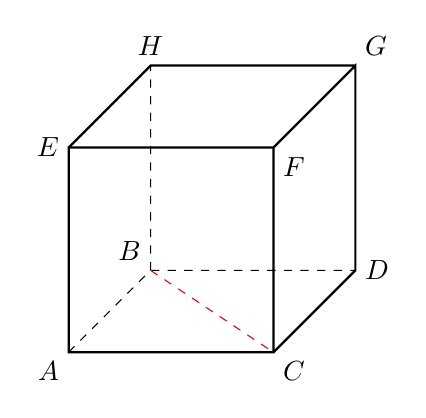
\begin{tikzpicture}[scale=1.3]
\coordinate (A) at (0,0); \coordinate (C) at (2,0); \coordinate (D) at (2.8,0.8); \coordinate (B) at (0.8,0.8);
\coordinate (E) at (0,2); \coordinate (F) at (2,2); \coordinate (G) at (2.8,2.8); \coordinate (H) at (0.8,2.8);
\draw[thick] (A) -- (C) -- (F) -- (E) -- cycle (C) -- (D) -- (G) -- (F) (E) -- (H) -- (G);
\draw[dashed] (A) -- (B) -- (D) (B) -- (H);
\draw[red,dashed] (B) -- (C);
\foreach \p/\a in {A/below left,C/below right,D/right,B/above left,E/left,F/below right,G/above right,H/above} \node[\a] at (\p) {$\p$};
\end{tikzpicture}
\end{center}
\begin{enumerate}[a]
  \item គេសង្កេតឃើញថា $BC$ និង $HG$ មិនស្ថិតក្នុងប្លង់តែមួយ ។ ប៉ុន្តែ $HG$ ស្របនឹង $BD$ ។ $BD$ និង $BC$ នៅក្នុងប្លង់តែមួយ និងមុំដែលបង្កើតឡើងដោយបន្ទាត់ទាំងពីរនេះគឺ $45^\circ$ ($BC$ ជាអង្កត់ទ្រូងនៃការេ $ACDB$) ។ ដូច្នេះ មុំដែលបង្កើតឡើងដោយអង្កត់ $BC$ និង $HG$ គឺ $45^\circ$ ។
  \item ដូចសំណួរ ក ដែរ គេបាន $CF \parallel BH$ ។ មុំដែលបង្កើតឡើងដោយអង្កត់ $BA$ និង $BH$ គឺ $90^\circ$ ។ ដូច្នេះ មុំដែលបង្កើតឡើងដោយគូអង្កត់ $BA$ និង $CF$ គឺ $90^\circ$ ។
\end{enumerate}
\end{example}

\begin{pro}
គេឱ្យ $I, J, K$ ជាចំណុចកណ្ដាលរៀងគ្នានៃជ្រុង $BC$, $AD$ និង $AC$ នៃតេត្រាអែត $ABCD$ ។
\begin{enumerate}[a]
  \item បង្ហាញថាមុំ $\angle I$ និង $\angle J$ នៃត្រីកោណ $IJK$ គឺជាមុំដែលបង្កើតឡើងដោយបន្ទាត់ $IJ$ ជាមួយនឹងបន្ទាត់ $AB$ និង $CD$ រៀងគ្នា ។
  \item បើ $AB = CD$ បង្ហាញថាត្រីកោណ $IJK$ ជាត្រីកោណសមបាត ។
\end{enumerate}
\ans
ក. ក្នុងត្រីកោណ $ABC$ ៖ $IK$ ជាបន្ទាត់កណ្ដាល ដូច្នេះ $IK \parallel AB$ ។ ក្នុងត្រីកោណ $ACD$ ៖ $JK \parallel CD$ ។ ហេតុនេះ $\angle KIJ$ ជាមុំរវាង $IJ$ និង $AB$ ហើយ $\angle IJK$ ជាមុំរវាង $IJ$ និង $CD$ ។ \quad ខ. $IK = \dfrac{AB}{2}$ និង $JK = \dfrac{CD}{2}$ ។ បើ $AB = CD$ នោះ $IK = JK$ ដូច្នេះ $IJK$ ជាត្រីកោណសមបាតកំពូល $K$ ។
\end{pro}

\subsection{ទីតាំងរវាងបន្ទាត់ និងប្លង់}
\begin{center}
\begin{tikzpicture}[scale=0.85]
\foreach \x in {0,4.6,9.2} {\draw[thick] (\x,0) -- (\x+3,0) -- (\x+3.8,1.3) -- (\x+0.8,1.3) -- cycle; \node at (\x+0.45,0.2) {\scriptsize $P$};}
\draw[red] (1.9,0.65) -- (1.9,2.2) node[right] {\scriptsize $d$}; \draw[red,dotted] (1.9,0.65) -- (1.9,0) ; \draw[red] (1.9,0) -- (1.9,-0.5); \fill (1.9,0.65) circle (1.5pt) node[left] {\scriptsize $A$};
\node at (1.9,-0.9) {\small $d \cap P = \{A\}$};
\draw[red] (4.6+0.6,1.9) -- (4.6+3.2,1.9) node[right] {\scriptsize $d$}; \node at (4.6+1.9,-0.9) {\small $d \parallel P$};
\draw[red] (9.2+1.0,0.4) -- (9.2+3.0,0.95) node[above] {\scriptsize $d$}; \node at (9.2+1.9,-0.9) {\small $d \subset P$};
\node at (1.9,2.6) {\small បន្ទាត់កាត់ប្លង់}; \node at (4.6+1.9,2.6) {\small បន្ទាត់ស្របប្លង់}; \node at (9.2+1.9,2.6) {\small បន្ទាត់នៅក្នុងប្លង់};
\end{tikzpicture}
\end{center}

\begin{example}[ឧទាហរណ៍]
បន្ទប់មួយរាងប្រលេពីប៉ែតកែង ($ABDC$ ជាបាត និង $EFHG$ ជាពិដាន ដែល $E, F, G, H$ នៅពីលើ $A, B, C, D$ រៀងគ្នា) ។ ប្រសិនបើគេជ្រើសរើសបន្ទាត់ $AB$ មួយ គេបាន ៖
\end{example}
\begin{itemize}
  \item បន្ទាត់ $AB$ កាត់ប្លង់ជញ្ជាំង $ACGE$ ត្រង់ $A$ ។ គេបាន $AB \cap ACGE = \{A\}$ ។
  \item បន្ទាត់ $AB$ ស្របនឹងប្លង់ពិដាន $EFHG$ ។
  \item បន្ទាត់ $AB$ នៅក្នុងប្លង់ $ABDC$ ។
\end{itemize}

\begin{pro}
តាមបីចំណុច $A, B, C$ រត់មិនត្រង់គ្នា គេគូសអង្កត់ $AA'$, $BB'$ និង $CC'$ ស្របគ្នាហើយប៉ុនគ្នា ។ $K, L, M, N, P$ ជាចំណុចកណ្ដាលរៀងគ្នានៃ $AB$, $A'C'$, $B'C'$, $KL$ និង $KM$ ។ បង្ហាញថា ៖
\begin{enumerate}[a]
  \item បន្ទាត់ $NP$ ប្រសព្វប្លង់ $AA'C'C$
  \item បន្ទាត់ $NP$ ប្រសព្វប្លង់ $BB'C'C$ ។
\end{enumerate}
\ans
ក្នុងត្រីកោណ $KLM$ ៖ $NP$ ជាបន្ទាត់កណ្ដាល ដូច្នេះ $NP \parallel LM$ ។ ក្នុងត្រីកោណ $A'B'C'$ ៖ $LM \parallel A'B'$ ។ ដូច្នេះ $NP \parallel A'B'$ ។ ក. បន្ទាត់ $A'B'$ កាត់ប្លង់ $AA'C'C$ ត្រង់ $A'$ ហើយ $NP$ ស្របនឹង $A'B'$ និងមិនស្ថិតក្នុងប្លង់នោះ ដូច្នេះ $NP$ ប្រសព្វប្លង់ $AA'C'C$ ។ \quad ខ. ដូចគ្នា $A'B'$ កាត់ប្លង់ $BB'C'C$ ត្រង់ $B'$ ដូច្នេះ $NP$ ប្រសព្វប្លង់ $BB'C'C$ ។
\end{pro}

\subsection{ទីតាំងរវាងប្លង់ពីរ}
\textbf{ប្លង់ត្រួតស៊ីគ្នា ៖} បើគ្រប់ចំណុចនៃប្លង់ $P$ ជាចំណុចរបស់ប្លង់ $Q$ នោះគេថា $P$ ត្រួតលើ $Q$ ។

\textbf{ប្លង់ស្របគ្នា ៖} បើប្លង់ពីរ $P$ និង $Q$ គ្មានចំណុចរួមនោះគេថា $P$ ស្របនឹង $Q$ ហើយគេសរសេរ $P \cap Q = \varnothing$ ឬ $P \parallel Q$ ។

\textbf{ប្លង់ប្រសព្វគ្នា ៖} បើប្លង់ពីរ $P$ និង $Q$ មិនត្រួតស៊ីគ្នា ឬមិនស្របគ្នានោះ ប្លង់ $P$ និង $Q$ ប្រសព្វគ្នាតាមបន្ទាត់ $\Delta$ មួយហើយគេសរសេរ $P \cap Q = \Delta$ ។
\begin{center}
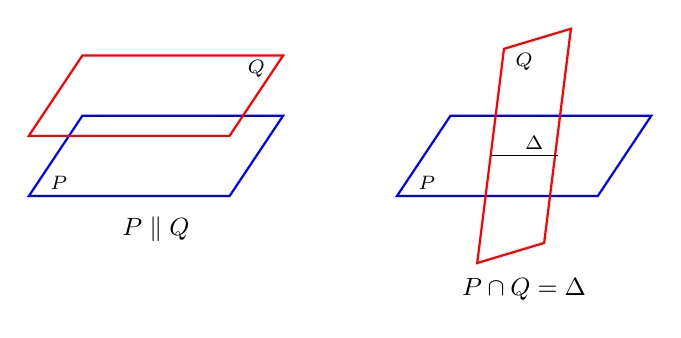
\begin{tikzpicture}[scale=0.85]
\draw[thick,blue] (0,0) -- (3,0) -- (3.8,1.2) -- (0.8,1.2) -- cycle; \node at (0.45,0.2) {\scriptsize $P$};
\draw[thick,red] (0,0.9) -- (3,0.9) -- (3.8,2.1) -- (0.8,2.1) -- cycle; \node at (3.4,1.9) {\scriptsize $Q$};
\node at (1.9,-0.5) {\small $P \parallel Q$};
\begin{scope}[xshift=5.5cm]
\draw[thick,blue] (0,0) -- (3,0) -- (3.8,1.2) -- (0.8,1.2) -- cycle; \node at (0.45,0.2) {\scriptsize $P$};
\draw[thick,red] (1.2,-1) -- (2.2,-0.7) -- (2.6,2.5) -- (1.6,2.2) -- cycle; \node at (1.9,2.0) {\scriptsize $Q$};
\draw (1.4,0.6) -- (2.4,0.6); \node at (2.05,0.8) {\scriptsize $\Delta$};
\node at (1.9,-1.4) {\small $P \cap Q = \Delta$};
\end{scope}
\end{tikzpicture}
\end{center}

\begin{example}[លំហាត់គំរូ]
គេមានប្រលេពីប៉ែតកែង $ABCDEFGH$ មួយ ($ABCD$ ជាមុខខាងក្រោម និង $EFGH$ ជាមុខខាងលើ ដែល $E, F, G, H$ នៅពីលើ $A, B, C, D$ រៀងគ្នា) ។
\begin{enumerate}[a]
  \item កំណត់ប្លង់ដែលស្របទៅនឹងប្លង់ $ABCD$
  \item កំណត់បន្ទាត់ប្រសព្វរវាងប្លង់ $ABCD$ និងប្លង់ $ACGE$ ។
\end{enumerate}
\ans
\begin{enumerate}[a]
  \item តាមរូបគេសង្កេតឃើញថាប្លង់ដែលស្របទៅនឹងប្លង់ $ABCD$ គឺប្លង់ $EFGH$ ៖ $ABCD \cap EFGH = \varnothing \Rightarrow ABCD \parallel EFGH$ ។
  \item ប្លង់ $ABCD$ ប្រសព្វ និងប្លង់ $ACGE$ បានបន្ទាត់ $AC$ ៖
  \[
  \left.\begin{aligned} AC &\subset ABCD\\ AC &\subset ACGE \end{aligned}\right\} \Leftrightarrow ABCD \cap ACGE = AC
  \]
\end{enumerate}
\end{example}

\begin{pro}
គេមានចតុមុខ $OABC$ ។ $M, N, P$ នៅលើជ្រុង $OA$, $OB$, $OC$ ។ បើប្លង់ $ABC$ មិនស្របនឹងប្លង់ $MNP$ ទេ ៖
\begin{enumerate}[a]
  \item សង់ប្រសព្វរវាងប្លង់ $ABC$ និង $MNP$ ។
  \item រកលក្ខខណ្ឌ $M, N, P$ ដើម្បីឱ្យប្លង់ $ABC \parallel MNP$ ។
\end{enumerate}
\ans
ក. តាង $I = MN \cap AB$ និង $J = NP \cap BC$ (ឬ $MP \cap AC$) ។ $I, J$ ជាចំណុចរួមនៃប្លង់ទាំងពីរ ដូច្នេះប្រសព្វគឺបន្ទាត់ $IJ$ ។ \quad ខ. $\dfrac{OM}{OA} = \dfrac{ON}{OB} = \dfrac{OP}{OC}$ ។
\end{pro}

\section*{លំហាត់អនុវត្តន៍}
\begin{enumerate}[1]
  \item $ABCDEFGH$ ជាប្រលេពីប៉ែតកែង ($ABCD$ ជាបាត, $H, G, F, E$ នៅពីលើ $A, B, C, D$ រៀងគ្នា) ហើយប្លង់ $MNPQ$ ស្របនឹងមុខ $ABCD$ ដែល $M \in CF$, $N \in DE$, $P \in AH$, $Q \in BG$ ។ បំពេញចម្លើយក្នុងចន្លោះ ៖ \quad ក. ប្លង់ $MPQ$ ប្រសព្វនឹងប្លង់ $ABG$ បានបន្ទាត់ ...... ។ \quad ខ. បន្ទាត់ $QM$ និង $BC$ ស្របគ្នា កាលណា $M$ និង $Q$ ជាចំណុចកណ្ដាលនៃជ្រុង ...... និង ...... រៀងគ្នា ។ \quad គ. បន្ទាត់ $PN$ និង $QM$ ស្របគ្នា កាលណា $M, N, P$ និង $Q$ ជាចំណុចកណ្ដាលនៃជ្រុង ......, ......, ...... និង ...... រៀងគ្នា ។
  \ans
  ក. $PQ$ \quad ខ. $CF$ និង $BG$ \quad គ. $CF$, $DE$, $AH$ និង $BG$ ។ (តាមពិត ដោយប្លង់ $MNPQ \parallel ABCD$ នោះ $QM \parallel BC$ និង $PN \parallel QM$ ជានិច្ច ។)
  \item សង់រូបនីមួយៗឡើងវិញ រួចដាក់អង្កត់ដាច់ៗនៃរូបខាងក្រោម ៖ ក. រូបប្រអប់មានរន្ធរាង U \quad ខ. រូបជណ្ដើរបីកាំ ។
  \ans
  គូសទ្រនុងដែលបាំង (មិនអាចមើលឃើញ) ដោយគំនូសដាច់ៗ និងរក្សាទ្រនុងស្របគ្នាឱ្យនៅស្របគ្នា ។
  \item សង់រូប ៖ \quad ក. ស្វ៊ែមួយ \quad ខ. ព្រីសត្រង់មួយដែលមានមុខខាងចំនួន $7$ \quad គ. ស៊ីឡាំងចារឹកក្នុងស្វ៊ែមួយ ដែលអង្កត់ផ្ចិតនៃស៊ីឡាំងនេះមានប្រវែងស្មើនឹងកម្ពស់របស់វា ។
  \ans
  ក. គូសរង្វង់មួយ និងអេលីបអេក្វាទ័រ (ពាក់កណ្ដាលខាងក្រោយគូសដាច់ៗ) ។ \quad ខ. ព្រីសដែលមានបាតជាពហុកោណ $7$ ជ្រុង ។ \quad គ. ស៊ីឡាំងមានកាំ $r$ និងកម្ពស់ $2r$ ចារឹកក្នុងស្វ៊ែកាំ $R = r\sqrt{2}$ ។
  \item គេឱ្យចតុមុខ $OABC$ មួយ ដែល $M$ ជាចំណុចកណ្ដាលនៃជ្រុង $OC$ និង $N, P$ ជាទីប្រជុំទម្ងន់នៃត្រីកោណ $\triangle OAC$, $\triangle OBC$ រៀងគ្នា ។ \quad ក. បង្ហាញថា $BM$ ប្រសព្វជាមួយនឹង $AP$ \quad ខ. រកលក្ខខណ្ឌនៃចំណុច $S$ ក្នុងត្រីកោណ $\triangle ABC$ ដើម្បីឱ្យ $OS$ ប្រសព្វជាមួយនឹង $NP$ ។
  \ans
  ក. $P$ ជាទីប្រជុំទម្ងន់នៃ $\triangle OBC$ ដូច្នេះ $P$ នៅលើមេដ្យាន $BM$ ។ ហេតុនេះ $AP$ និង $BM$ ស្ថិតក្នុងប្លង់ $ABM$ តែមួយ ហើយប្រសព្វគ្នាត្រង់ $P$ ។ \quad ខ. តាង $I, J$ ជាចំណុចកណ្ដាលនៃ $AC$ និង $BC$ ។ $N \in OI$ និង $P \in OJ$ ($ON = \tfrac{2}{3}OI$, $OP = \tfrac{2}{3}OJ$) ដូច្នេះប្លង់ $ONP$ កាត់ប្លង់ $ABC$ តាមបន្ទាត់ $IJ$ ។ $OS$ ប្រសព្វ $NP$ លុះត្រាតែ $S$ ស្ថិតនៅលើអង្កត់ $IJ$ (បន្ទាត់កណ្ដាលនៃ $\triangle ABC$ ស្របនឹង $AB$) ។
  \item គេមានចំណុច $B, C$ ស្ថិតក្នុងប្លង់ $P$ មួយ និងចំណុច $A$ មិនស្ថិតក្នុងប្លង់ $P$ ។ ដៅចំណុច $M$ មួយជារបស់ប្លង់ $ABC$ រួចបន្លាយ $AM$ កាត់ប្លង់ $P$ ត្រង់ $N$ ។ បង្ហាញថា $B, C, N$ ស្ថិតលើបន្ទាត់តែមួយ ។
  \ans
  $N \in AM \subset ABC$ និង $N \in P$ ។ ចំណុច $B, C$ ក៏ស្ថិតក្នុងប្លង់ទាំងពីរ $ABC$ និង $P$ ដែរ ។ ប្លង់ទាំងពីរខុសគ្នា ($A \notin P$) ដូច្នេះវាប្រសព្វគ្នាតាមបន្ទាត់តែមួយ គឺបន្ទាត់ $BC$ ។ ហេតុនេះ $B, C, N$ ស្ថិតលើបន្ទាត់តែមួយ ។
\end{enumerate}
